\chapter{Reti neurali randomizzate}\label{ch-18}

Dopo il deep learning, l'altro paradigma recente presentato nel corso è
quello delle \textbf{reti neurali a pesi casuali} (``deep learning ed
\emph{extreme} learning'', scherza il professore). L'idea sembra
paradossale: e se lo strato nascosto non venisse addestrato affatto? La
lezione mostra come la casualità sia una componente utile del ML e come
le reti randomizzate si ricolleghino a concetti già visti: espansione in
basi, teorema di Cover, regolarizzazione.

\section{La casualità nel Machine
Learning}\label{la-casualituxe0-nel-machine-learning}

Un approccio \textbf{randomizzato} usa un certo grado di casualità come
parte della sua strategia costruttiva. La casualità può migliorare le
prestazioni predittive e alleviare le difficoltà delle metodologie
classiche, ed è presente a diversi livelli:

\begin{itemize}
\tightlist
\item
  \textbf{elaborazione dei dati}: suddivisione dei dati (hold-out,
  K-fold CV, leave-one-out), generazione di dati (bootstrap, boosting,
  tecniche di bilanciamento);
\item
  \textbf{apprendimento}: ordine delle osservazioni (shuffling per il
  mini-batch), inizializzazione casuale dei pesi delle reti;
\item
  \textbf{selezione degli iperparametri} (inclusa la ricerca casuale);
\item
  \textbf{ensemble}: differenziazione casuale tra modelli
  (inizializzazioni diverse, campionamento dei training set in bagging e
  boosting);
\item
  \textbf{nel cuore del modello}.
\end{itemize}

\subsection{Modelli intrinsecamente
casuali}\label{modelli-intrinsecamente-casuali}

\begin{itemize}
\tightlist
\item
  I neuroni stocastici delle \textbf{Restricted Boltzmann Machine}.
\item
  Gli \textbf{Extremely Randomized Trees} e le \textbf{Random Forest}:
  un ensemble di alberi di decisione randomizzati, ciascuno costruito su
  campioni estratti casualmente dal training set e con una scelta
  casuale delle variabili di input su cui dividere i nodi. Uniscono i
  vantaggi degli ensemble e della casualità.
\item
  Il \textbf{dropout} come regolarizzazione (anche se qui la casualità
  non è necessaria di per sé).
\end{itemize}

\begin{figure}[htbp]
\centering
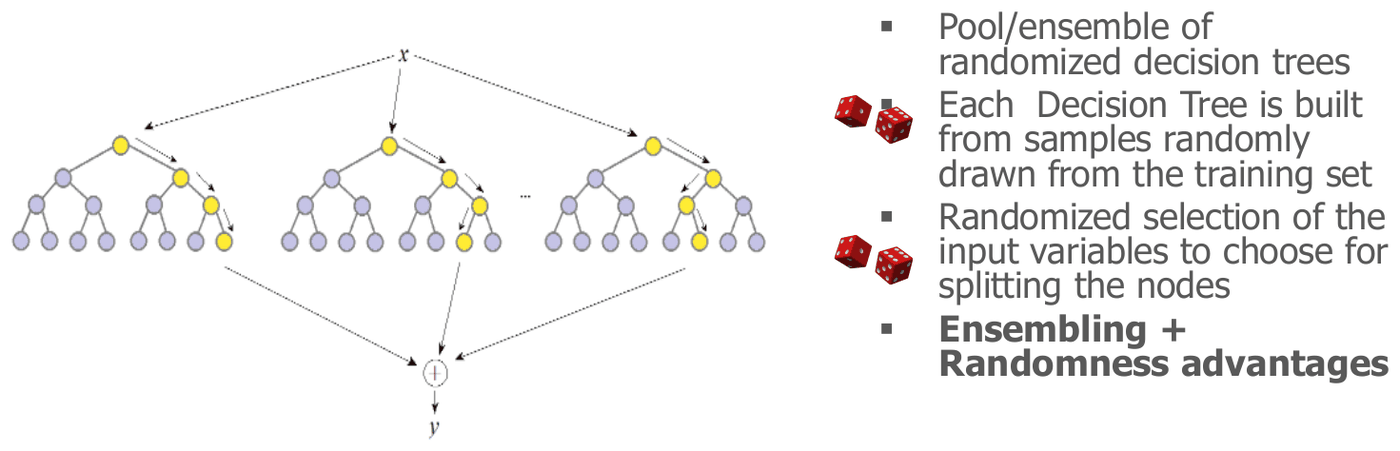
\includegraphics[width=0.71\linewidth,height=0.42\textheight,keepaspectratio]{images/18-rand_random-forest.png}
\caption{Random Forest: un ensemble di alberi di decisione randomizzati.}
\end{figure}

\section{Reti neurali a pesi casuali}\label{reti-neurali-a-pesi-casuali}

\begin{boxquestion}{La domanda}

È possibile sfruttare le architetture MLP (o ricorrenti) \textbf{senza
lunghi cicli di addestramento} degli strati nascosti?

\end{boxquestion}

Esiste una lunga tradizione di reti randomizzate, a pesi casuali, a
proiezione casuale: ad esempio la \textbf{Random Vector Functional Link}
(RVFL), fin dalle origini. Di recente sono state rese popolari con vari
nomi, tra cui \textbf{ELM} (\emph{Extreme Learning Machine}).

\begin{boxdefinition}{Idea di base}

\begin{itemize}
\tightlist
\item
  Una rete con uno (o più) \textbf{strati nascosti connessi
  casualmente}: i pesi vengono \textbf{fissati dopo l'inizializzazione
  casuale} e non vengono più addestrati.
\item
  Si addestrano \textbf{solo i pesi di uscita} (un modello lineare: con
  la pseudoinversa o la ridge regression).
\end{itemize}

Si superano così i problemi degli algoritmi di addestramento complessi e
computazionalmente onerosi tradizionalmente usati per le reti neurali.

\end{boxdefinition}

Le radici sono nel lavoro pionieristico sul \textbf{Perceptron} di
Rosenblatt, in cui un'area di ``proiezione'' connessa casualmente alla
retina alimentava un'area di ``associazione'', e solo le risposte finali
venivano apprese. Altri lavori pionieristici avevano sottolineato
l'importanza dell'apprendimento nello strato di uscita rispetto a quello
nascosto.

\begin{figure}[htbp]
\centering
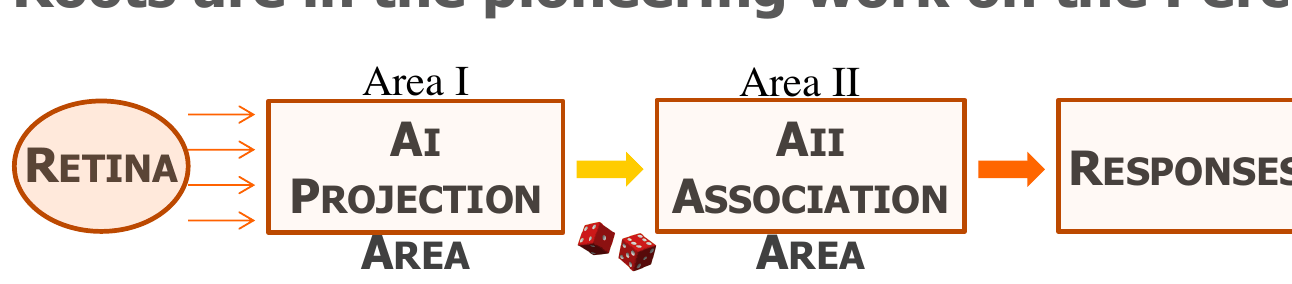
\includegraphics[width=0.69\linewidth,height=0.42\textheight,keepaspectratio]{images/18-rand_perceptron.png}
\caption{Il Perceptron originale: le connessioni dalla retina all'area di
proiezione erano casuali.}
\end{figure}

Le reti randomizzate sono oggi una linea di ricerca in crescita,
particolarmente adatta quando l'\textbf{efficienza} è fondamentale
(l'addestramento è limitato all'ultimo strato).

\subsection{Struttura generale}\label{struttura-generale}

\begin{figure}[htbp]
\centering
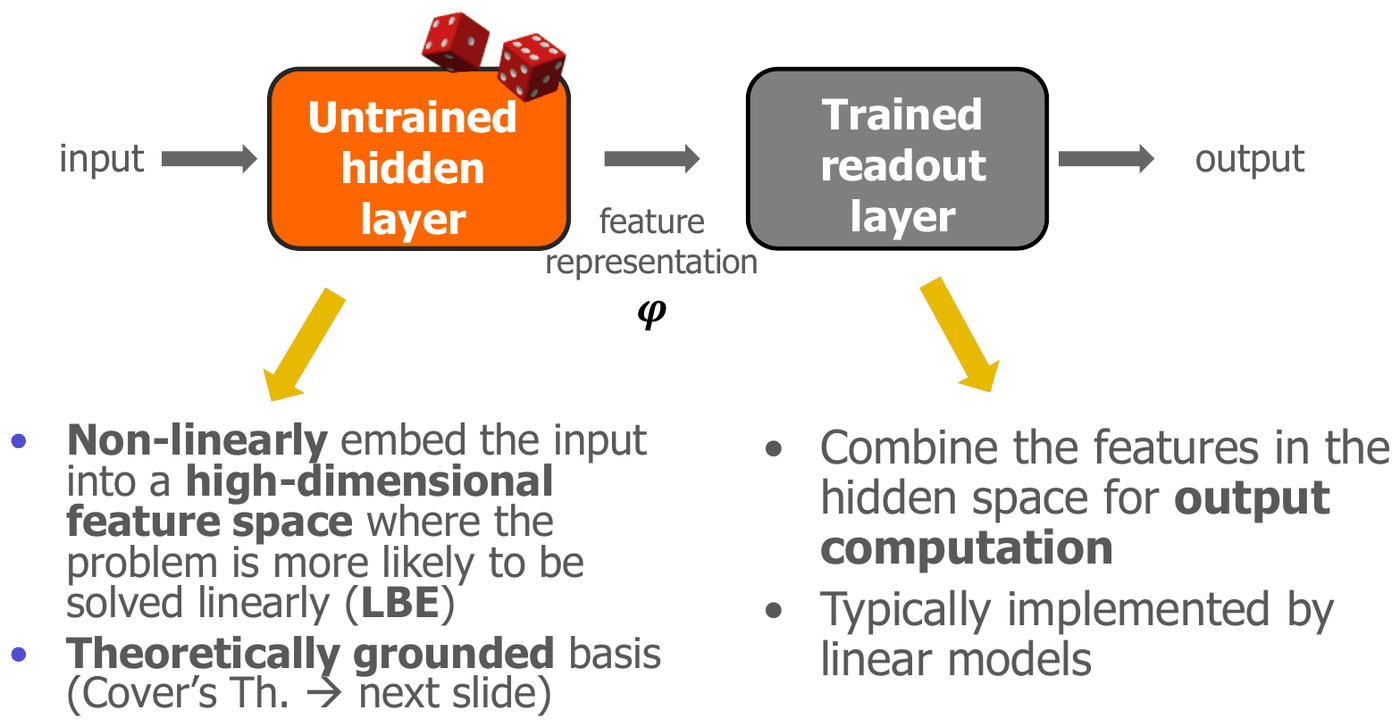
\includegraphics[width=0.80\linewidth,height=0.42\textheight,keepaspectratio]{images/18-rand_struttura.png}
\caption{Struttura generale: uno strato nascosto non addestrato (casuale) e uno
strato di readout addestrato.}
\end{figure}

\begin{itemize}
\tightlist
\item
  \textbf{Strato nascosto (non addestrato)}: immerge in modo \textbf{non
  lineare} l'input in uno \textbf{spazio delle feature ad alta
  dimensione}, dove il problema ha più probabilità di essere risolvibile
  linearmente (è una \textbf{LBE}!). Ha una base teorica nel teorema di
  Cover.
\item
  \textbf{Readout (addestrato)}: combina le feature dello spazio
  nascosto per calcolare l'uscita; tipicamente è un \textbf{modello
  lineare}.
\end{itemize}

\begin{boxtheorem}{Teorema di Cover (1965)}

\emph{``Un problema complesso di classificazione di pattern, proiettato
in modo non lineare in uno spazio ad alta dimensione, ha più probabilità
di essere linearmente separabile che in uno spazio a bassa dimensione,
purché lo spazio non sia densamente popolato.''}

Ad esempio, con una mappatura deterministica: dati \(l\) esempi, li si
solleva sui vertici di un simplesso \((l-1)\)-dimensionale (il
``triangolo'' generalizzato). Ora \textbf{ogni} partizione binaria dei
campioni è linearmente separabile.

\end{boxtheorem}

È esattamente la stessa proprietà sfruttata dai \textbf{kernel} nelle
SVM.

\subsection{Reti feedforward
randomizzate}\label{reti-feedforward-randomizzate}

\begin{figure}[htbp]
\centering
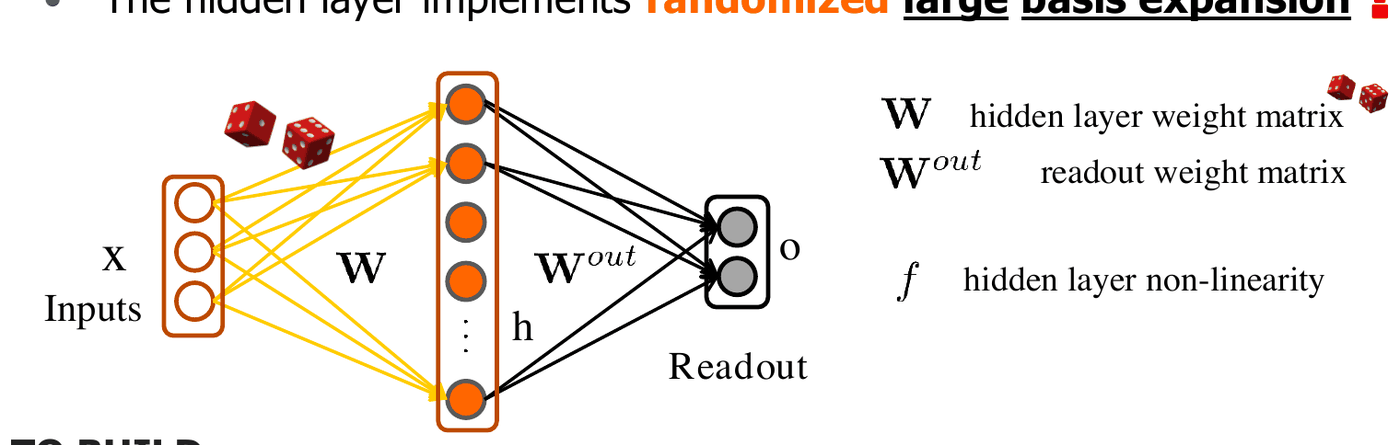
\includegraphics[width=0.80\linewidth,height=0.42\textheight,keepaspectratio]{images/18-rand_rete.png}
\caption{Rete feedforward randomizzata: \(\mathbf{W}\) (casuale, fissa) e
\(\mathbf{W}^{out}\) (addestrata).}
\end{figure}

La relazione input-output è implementata da uno strato nascosto non
addestrato, che realizza una \textbf{grande espansione in basi casuale}.

\begin{boxabstract}{Costruzione, apprendimento e uso}

\textbf{Costruzione}: riempire \(\mathbf{W}\) con valori casuali (ad
esempio rumore gaussiano), usando \textbf{molte unità}.

\textbf{Apprendimento} del readout: dati \(l\) esempi
\((\mathbf{x}_p, \mathbf{d}_p)\), come per i modelli lineari si
minimizza l'errore quadratico con il metodo diretto. Con
\(\mathbf{H} = f(\mathbf{W}\mathbf{X})\) (le attivazioni nascoste di
tutti i pattern): \[
\mathbf{W}^{out} = \mathbf{H}^+\mathbf{d},
\] spesso con \textbf{regolarizzazione \(L^2\)} (utile per l'alto numero
di unità): \[
\mathbf{W}^{out} = (\mathbf{H}^T\mathbf{H} + \lambda\mathbf{I})^{-1}\mathbf{H}^T\mathbf{d},
\] oppure con \(L^1\).

\textbf{Uso}: si calcolano le attivazioni nascoste \(\mathbf{h}\) come
per i normali neuroni e poi le uscite \[
\mathbf{o}(\mathbf{x}) = \mathbf{W}^{out} f(\mathbf{W}\mathbf{x}),
\] applicando eventualmente una soglia (o una funzione non lineare) per
la classificazione.

\end{boxabstract}

I principali modelli di riferimento sono la \textbf{RVFL} (\emph{Random
Vector Functional-Link}), la \textbf{ELM} (\emph{Extreme Learning
Machine}) e le \textbf{reti RBF con centri casuali}.

\begin{boxtip}{Perché funziona}

Si confronti con le reti neurali ``normali'': lì lo strato nascosto è
un'espansione in basi \textbf{adattiva}
\(\phi_j(\mathbf{x}, \mathbf{w})\) i cui pesi vengono appresi; qui è
un'espansione in basi \textbf{casuale} ma molto \textbf{ampia}. Se le
basi sono abbastanza numerose, per il teorema di Cover il problema
diventa (quasi) linearmente separabile nello spazio nascosto, e basta un
modello lineare in uscita, addestrabile in un solo passo con i minimi
quadrati. Il costo di addestramento è quello di una regressione lineare
regolarizzata.

\end{boxtip}

\subsection{Pro e contro}\label{pro-e-contro}

\begin{itemize}
\tightlist
\item
  Il grande insieme di unità nascoste ha un ruolo interessante: la
  proiezione espande in modo non lineare la dimensione dell'input,
  rendendo i dati più separabili.
\item
  Un numero elevato di unità può fornire un'espansione in basi
  \textbf{sufficiente} per il task (con basi teoriche, inclusi teoremi
  di approssimazione universale).
\item
  \textbf{Estremamente efficienti}.
\item
  Esistono molte varianti: apprendimento incrementale aggiungendo
  neuroni (come il Cascade Correlation), pruning, ecc., spesso legate a
  ricerche passate con nomi diversi.
\item
  Modelli ``mirati'', con meno unità adattive addestrate sul task
  specifico, sembrano comunque \textbf{più eleganti}: c'è un dibattito
  tra approcci a \textbf{feature casuali} e a \textbf{feature apprese},
  e vale la pena conoscerli entrambi.
\item
  Si estendono alle reti ricorrenti: le \textbf{Echo State Network}
  (ESN), vedi
  \href{20\%20-\%20Reti\%20neurali\%20ricorrenti\%20(RNN)}{20 - Reti
  neurali ricorrenti (RNN)}.
\end{itemize}

\subsection{Dove sono utili}\label{dove-sono-utili}

\begin{itemize}
\tightlist
\item
  \textbf{Big Data}, grazie all'efficienza estrema.
\item
  Implementazioni minuscole per sistemi \textbf{embedded} e distribuiti,
  su dispositivi con risorse limitate (reti di sensori, IoT, edge
  computing).
\item
  \textbf{Deep learning}, dove gli algoritmi di addestramento sono
  particolarmente onerosi: le reti randomizzate alleviano il carico
  computazionale (reti profonde randomizzate come pile di moduli
  RVFL/ELM, CNN randomizzate).
\item
  \textbf{Reti ricorrenti randomizzate}: dove l'addestramento è ancora
  più oneroso che per gli MLP, e con solide basi teoriche sul bias
  introdotto dalla dinamica del sistema (stabilità, apprendibilità).
\end{itemize}

\begin{boxabstract}{Conclusioni}

\textbf{La casualità non è un nemico: è un'amica, se la si controlla.}
(Vale anche in altri campi dell'informatica, come gli algoritmi
randomizzati, e in matematica.) Si noti come ritornino sempre gli stessi
concetti --- teorema di Cover, LBE, regolarizzazione, rappresentazione
delle feature: il corso è ormai ``maturo''.

\end{boxabstract}

\begin{boxnote}{FAQ: si possono usare le ELM nel progetto?}

Sì, ma come \textbf{parte aggiuntiva} rispetto all'implementazione
standard di un MLP addestrato completamente con backpropagation e SGD.
Sono facili da implementare come sotto-parte di una rete feedforward.

\end{boxnote}

\begin{boxquestion}{Possibili domande d'esame}

\begin{itemize}
\tightlist
\item
  A quali livelli compare la casualità nel ML?
\item
  Descrivere una rete feedforward randomizzata: costruzione,
  addestramento del readout, uso.
\item
  Enunciare il teorema di Cover e spiegarne il legame con le reti
  randomizzate e con i kernel.
\item
  Pro e contro delle feature casuali rispetto alle feature apprese.
\end{itemize}

\end{boxquestion}
